\chapter{Introduction}
Fitting is the process of generating a 3D model of a face from a 2D image. There are different approaches on how to do that. The gravis group of the University of Basel has developed an MCMC (Markov Chain Monte Carlo) algorithm that makes random changes to a 3DMM (3D Morphable Model) and accepts the proposal face whenever the new 3D face has a greater probability than the previous one. For this Thesis, we use the popular Basel Face Model 2017 \cite{BFM2017}. That the algorithm can determine the likelihood of a 3D facial proposal relative to a given 2D face, the algoritm's evaluator needs to now, which pixels to include in the probability calculation. Therefore we have to label each pixel if it's part of the face which should be regarded by the evaluator, or if it's background and hsn't any importance for the construction of the 3D Model. Nirkin et al \cite{nirkin2018_faceswap} claim, that this is possible with a standart fully convolutional network.\\ 
\\
The idea of Artificial Neural Networks was heavily influenced by biology. They consist of a variety of neurons which are grouped in layers. The way each neuron works is very simple. It takes multiple inputs of varying strength from other neurons, sums them up and decides depending on the sum whether it should send a stimulus itself and if so, in which strength. Each layer is somehow connected to the next layer. Some layers are fully connected (each neuron of a layer is connected to every other neuron in the next layer) while others are convolutional. Convolutional means that a neuron only gets input of its neighbors in a previous layer. There are many different architectures which mainly differ in the number of layers, number of neurons per layer and the interconnectivity of the neurons. A classical Convolutional Neural Network (CNN) is depicted in \ref{fig:test1}.\\
\\
\begin{figure}
	\centering
	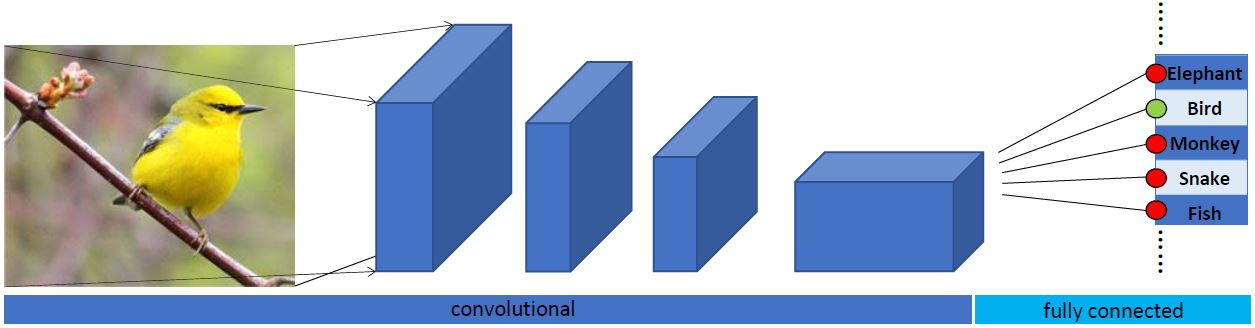
\includegraphics[width=1\linewidth]{Figures/chap1/classicalCNN.JPG}
	\caption{In the lower-left corner, you see the 16 layers of the VGG16-FCN. Each Max-Pooling layer cuts the input image size in half. In the top-right, you can see the meaning of the '8s' term of the FCN-Name. It means that the resulting image has to be 8x upsampled, to get an image which is in size equal to the input image (which means we have four pooling-layers)}
	\label{fig:test1}
\end{figure}

Already in 1943 Warren McCulloch and Walter Pitts \cite{mcculloch} showed that even simple networks of this kind can simulate every possible logical formula. For this they used a neuron model that consisted of simple logic gates and could process only binary input and output signals.

\begin{figure}[h]
	\centering
	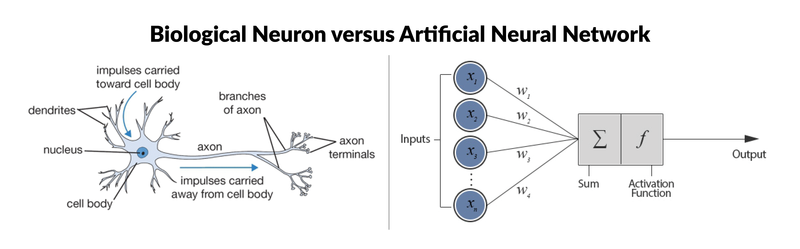
\includegraphics[width=1\linewidth]{Figures/chap1/bio_vs_arti_neuron.png}
	\caption[Caption for LOF]{The left-hand side of the image \footnotemark shows a Biological Neuron. It is a nerve cell that occurs in almost every animal. On the right-hand side is On the right is an artificial neuron. It sums up the stimuli of the previous neurons, applies an activation function to this sum and forwards the output of this function itself}
	\label{fig:test1}
\end{figure}

\footnotetext{Source: Google.com}

\section{Adjustment of the edgeweights}
The algorithm for this is called \textit{backpropagation}. To train a network, the desired output must be known. Depending on the difference between the actual output and the desired output, the new weight of each edge is determined by derivation. For details see \ref{subs:Example}

\lipsum[1]


\begin{figure}[h]
	\centering
	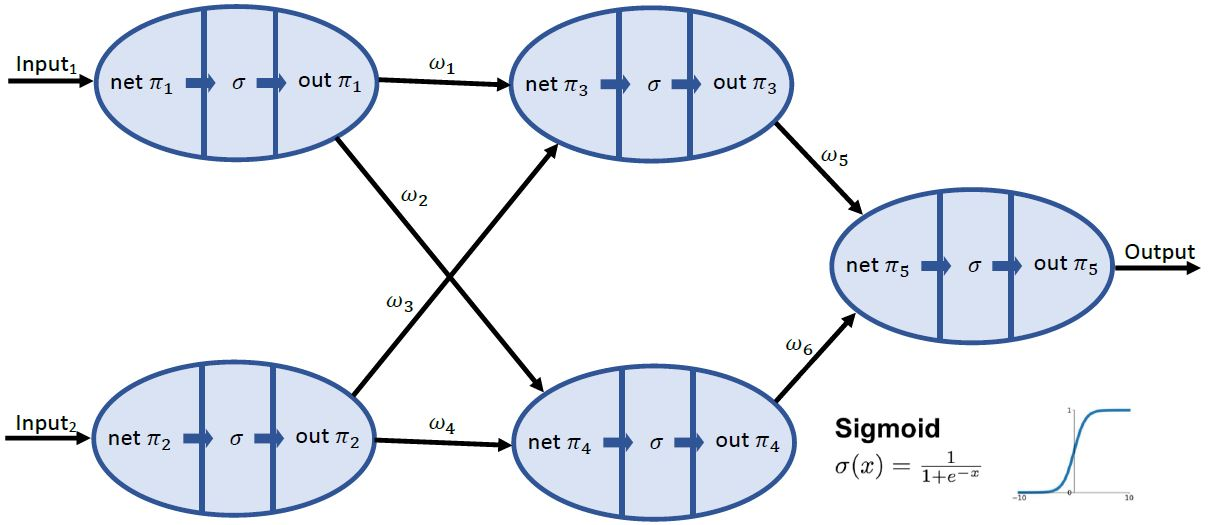
\includegraphics[width=1\linewidth]{Figures/chap1/backpropagation_example.JPG}
	\caption{A simple neural network consisting of three layers. Neurons $\pi_1$ and $\pi_2$ are in the input layer. $\pi_3$ and $\pi_4$ make up the only hidden layer and $\pi_5$ is in the output layer. Each neuron sums up the input signals ($net\pi_i$), applies an activation function to it ($\sigma$) and forwards the output of this function as its own signal ($out\pi_i$). Mostly a sigmoid function is choosen as the activation function (right lower corner). The edgeweights are annotated with $\omega_i$.}
	\label{fig:backpropagation}
\end{figure}

\subsection{A simple claculation example (on Figure \ref{fig:backpropagation})}
\label{subs:Example}

For this example, we assume that the neuron (and the edge connected to it) labeled with $\omega_1$ is in the input layer and the $\omega_3$ neuron is in the output layer. The layer where $\omega_2$ is in, is called \textit{hidden layer}. For this example, the inputs and edgeweights are as follows:
\begin{itemize}
	\item $Input_1$: 1
	\item $Input_2$: 0
	\item $\omega_i=\frac{i}{10}\forall i \in \{1,...,6\}$
\end{itemize}
First, let's calculate the output ($out\pi_5$) of the network:

\noindent\begin{minipage}{.5\linewidth}
	\begin{align*} 
		out\pi_1 &= \frac{1}{1+e^{-1}} = 0.731 \\ 
		out\pi_2 &= \frac{1}{1+e^{-0}} = 0.5 \\
		net\pi_3 &= 0.1*0.731+0.3*0.5 = 0.223 \\
		net\pi_4 &= 0.4*0.5+0.2*0.731 = 0.346
	\end{align*}
\end{minipage}%
\begin{minipage}{.5\linewidth}
	\begin{align*} 
		out\pi_3 &= \frac{1}{1+e^{-0.223}} = 0.556 \\ 
		out\pi_4 &= \frac{1}{1+e^{-0.346}} = 0.586 \\
		net\pi_5 &= 0.5*0.556+0.6*0.586 = 0.630 \\
		out\pi_5 &= \frac{1}{1+e^{-0.630}} = 0.652
	\end{align*}
\end{minipage}\\
\\
\\
The output of the network is $0.652$, but we want it to be $0.1$. Since $\sigma^{-1}(0.1)=-ln(9)$ we expect both $\omega_5$ and $\omega_6$ to get smaller. For the backpropagation we need an error-function. We choose the MSE (mean squared error). So $MSE=(0.652-0.1)^2 = 0.305$. We start the backpropagation calculation with applaying the chain rule to the derivative of the error with respect to the edgeweight which has to be updated:
\begin{equation*}
	\omega_i^* = \omega_i+\Delta \omega_i=\omega_i+\frac{\partial MSE}{\partial \omega_i}=\omega_i+\underbrace{\frac{\partial MSE}{\partial out\pi_5}*\frac{\partial out\pi_5}{\partial net\pi_5}}_{\delta_{\pi_5}}*\frac{\partial net\pi_5}{\partial \omega_i} \text{ for }i \in \{5,6\}
\end{equation*}
\begin{itemize}
	\item $\delta_{\pi_5}=\frac{\partial MSE}{\partial out\pi_5}*\frac{\partial out\pi_5}{\partial net\pi_5}=2*(0.652-0.1)*-1*0.652*(1-0.652)=-0.2505$
	\item $\omega_5^*=\omega_5+\delta_{\pi_5}*\frac{\partial net\pi_5}{\partial \omega_5}=\omega_5+\delta_{\pi_5}*out\pi_3=0.361$
	\item $\omega_6^*=\omega_6+\delta_{\pi_5}*\frac{\partial net\pi_5}{\partial \omega_6}=\omega_6+\delta_{\pi_5}*out\pi_4=0.453$
\end{itemize}
Now we move on with the $\Delta\omega_i$'s for the \textit{hidden layer}:
\begin{equation*}
	\frac{\partial E}{\partial \omega_i}=\underbrace{\underbrace{\frac{\partial MSE}{\partial out\pi_5}*\frac{\partial out\pi_5}{\partial net\pi_5}}_{\delta\pi_5}*\underbrace{\frac{\partial net\pi_5}{\partial out\pi_3}}_{\omega_5}*\frac{\partial out\pi_3}{\partial net\pi_3}}_{\delta_{\pi_3}}*\frac{\partial net\pi_3}{\partial \omega_i}\text{ for }i\in\{1,3\}
\end{equation*}
\begin{equation*}
	\frac{\partial E}{\partial \omega_i}=\underbrace{\underbrace{\frac{\partial MSE}{\partial out\pi_5}*\frac{\partial out\pi_5}{\partial net\pi_5}}_{\delta\pi_5}*\underbrace{\frac{\partial net\pi_5}{\partial out\pi_4}}_{\omega_6}*\frac{\partial out\pi_4}{\partial net\pi_4}}_{\delta_{\pi_4}}*\frac{\partial net\pi_4}{\partial \omega_i}\text{ for }i\in\{2,4\}
\end{equation*}

\noindent\begin{minipage}{.5\linewidth}
	\begin{align*} 
		\delta_{\pi_3} &= \delta_{\pi_5}*\omega_5^*out\pi_3*(1-out\pi_3)=-0.022\\ 
		\omega_1^* &= \omega_1+\delta_{\pi_3}*out\pi_1=0.084 \\
		\omega_3^* &= \omega_3+\delta_{\pi_3}*out\pi_2=0.289
	\end{align*}
\end{minipage}%
\begin{minipage}{.5\linewidth}
	\begin{align*} 
		\delta_{\pi_4} &= \delta_{\pi_5}*\omega_6^*out\pi_4*(1-out\pi_4)=-0.028\\ 
		\omega_2^* &= \omega_2+\delta_{\pi_4}*out\pi_1=0.180 \\
		\omega_4^* &= \omega_4+\delta_{\pi_4}*out\pi_2=0.386
	\end{align*}
\end{minipage}\\
\\
If we now evaluate the network, we get a $out\pi_5$ of $0.613$. This is a very small change in absolute values because we have made only one iteration of the backpropagation algorithm. However the MSE improves from $0.305$ to $0.263$!

\section{The network used}
\label{sec:theFCN}
For this thesis, we used a pretrained fully convolutional network from \cite{nirkin2018_faceswap}. A Fully Convolutional Network (often called: FCN) is basically a CNN but with a modified architecture. An FCN doesn't have the fully connected layers usually found at the end of an CNN. These layers would enable the Network to make decisions based on global information. Aa CNN can for example be used for classification. But for image analysis we want local information of the input image (we don't want to know if there is a face in the image, but where the face is in the image). Therefore a FCN uses only convolutional and pooling layers. In the whole Fully Convolutional Network only the following structure is repeated: One or more convolution layers and a pooling layer which downsamples the picture. This constellation is repeated several times.\\
\\
The assembly of our network used for this thesis follows the FCN-8s-VGG architecture with extensions of \cite{jlong}. The first part 'FCN' stands for 'fully convolutional network', '8s' means that the result gets eight times upsampled (4 pooling layers) and 'VGG' means the popular 16-layer network used by Oxford's Visual Geometry Group \cite{ksimonyan}. The original task of the network was to find the name of an object in an input image. The network could distinguish between 1000 different objects. Each cell in the final Softmax-Layer (1*1000 in size) was a boolean variable for one specific object.

\begin{figure}
	\centering
	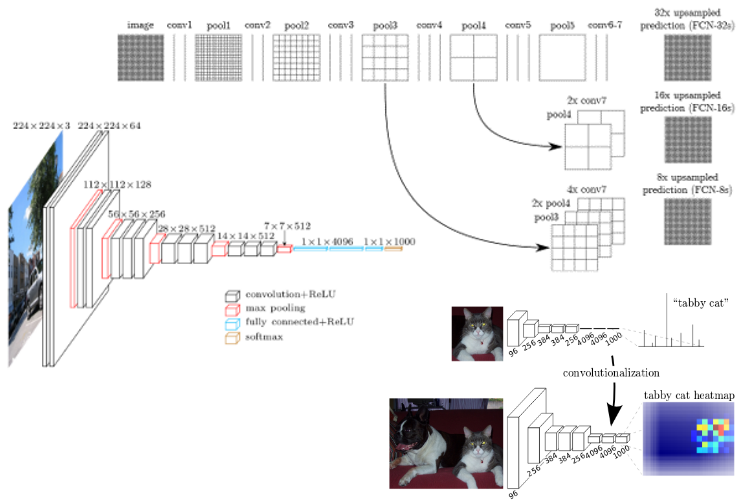
\includegraphics[width=1\linewidth]{Figures/fcn_1.png}
	\caption{In the lower-left corner, you see the 16 layers of the VGG16-FCN. Each Max-Pooling layer cuts the input image size in half. In the top-right, you can see the meaning of the '8s' term of the FCN-Name. It means that the resulting image has to be 8x upsampled, to get an image which is in size equal to the input image (which means we have four pooling-layers)}
\end{figure}


\section{Related Work}
For our experiments we used a pretrained Fully Convolutional Network (FCN) of \cite{nirkin2018_faceswap}. They showed that even with a widespread network, you can do good segmentation and that the network does not have to be specially tailored to the future purpose. But the network must have been trained with a large enough data set. For more details about the used FCN and the architecture see section \ref{sec:theFCN}. They used the FCN for intra- and intersubject face swapping on the Labeled Faces in the Wild (LFW) data set and showed that intra-subject swapped faces remain as recognizable as before the swap and that in the intersubject version better face swapping  leads to less perceptibility.\\
\\
They used a semi-supervised approach to produce training data in order to train the FCN. To produce large quantities of them, they used 2'043 face videos of the IARPA Janus CS2 dataset. To avoid searching for the face in every frame of the video they used motion queues which tracked the face based on an initial segmentation based on \cite{grundmann} which enriched their trainingset to 9'818 images. To enlarge the collection of images, they rendered 3D Shapes of of various objects (e.g. sunglasses, hands) into existing images. Each occlusion added 9'500 images to their trainingset.\\
\\
The gravis group of the University of Basel developped "Occlusion Aware 3D Morphable Models" \cite{egger_paper}. These Methods use an iterative approach to generate the z-labels, namely to label each pixel wether it belogs to the face or is background. This approach can handle multiple labels and differentiate between multiple occlusion types. For example face specific ones (eg. beards, sunglasses) and background. For updating the z-labels they use an algorithm which classifies a pixel based on the probabilities for each possible label.  But for our experiments we limited ourselves to two. We only need to distinguish face (including skin and beard) and background.\\ 
\\
The algorithm does two things at the same time. In addition to creating a face mask, it estimates a 3D reconstruction of the depicted face. It's an EM-algorithm like method to solve two problems simultaneusly. In the E-steps they updated the z-labels and in the M-steps they updated the face parameters. Conventional approaches often fail on important parts of the face such as the eyes, eyebrows or the oral region because oftheyr strong variability in color and shape. The segmentation of \cite{egger_paper} also has difficulties with these aspects as Figure \ref{fig:iterations} shows. The algorithm starts with an initial guess and then altenating updates the Parameters $\Theta$ and the z-labels. From the updated Parameter Set (M-Step) the algorithm updates the z-labels (E-Step) and vice versa (see Figure \ref{fig:EGGER's_method}).\\
\\
% Soll ich auch die 'stable illumination estimation' in ein chapter machen? Wenn ja, was ist das 'consensus set' ?

% The source for this table was this post: https://stackoverflow.com/questions/2771856/centering-text-horizontally-and-vertically-in-latex
% To add padding for the cell contents: https://tex.stackexchange.com/questions/31672/column-and-row-padding-in-tables
\begin{figure}[h]
	\begin{center}
		\newcolumntype{C}{>{\centering\arraybackslash} m{3cm} }  %# New column type
		\begin{tabular}{SC|SC|SC|SC}
			 target image & initial segmentation & after 10 iterations & after 20 iterations\\ \hline
			\subfloat{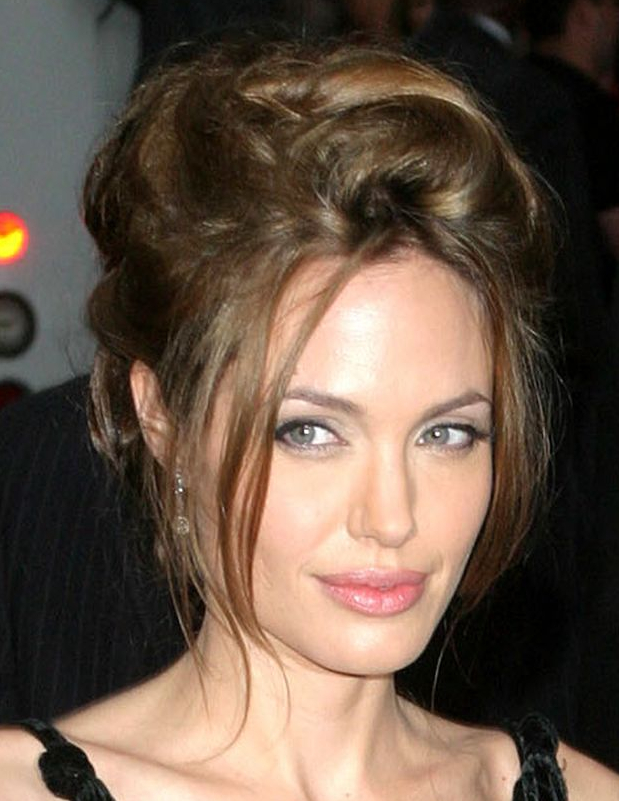
\includegraphics[width=0.2\textwidth]{Figures/chap1/angie_original.png}} &
			\subfloat{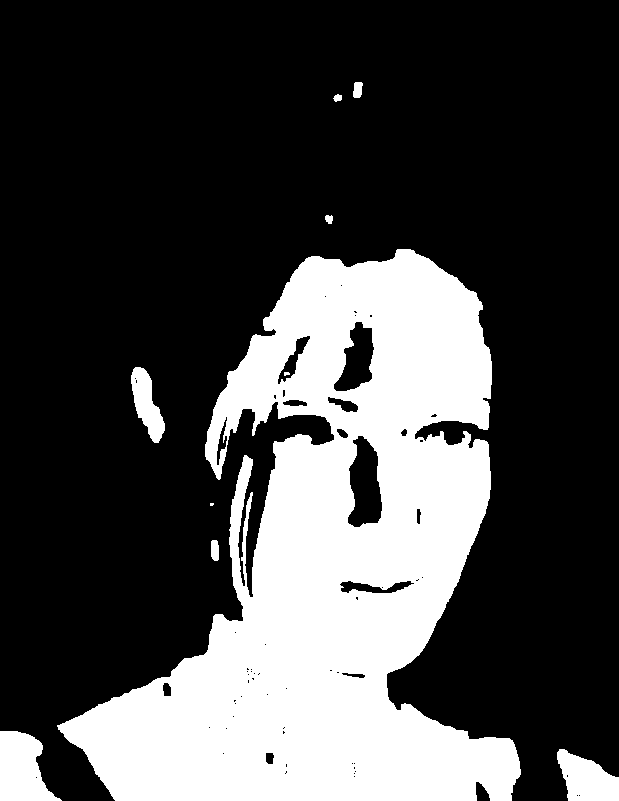
\includegraphics[width=0.2\textwidth]{Figures/chap1/EGGER_Segmentation_Nr_0.png}} &
			\subfloat{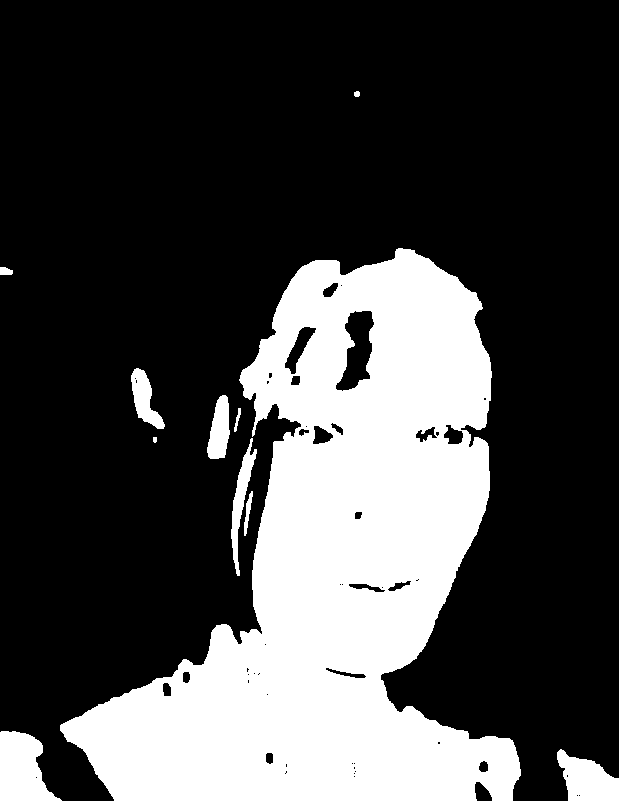
\includegraphics[width=0.2\textwidth]{Figures/chap1/EGGER_Segmentation_Nr_9.png}} &
			\subfloat{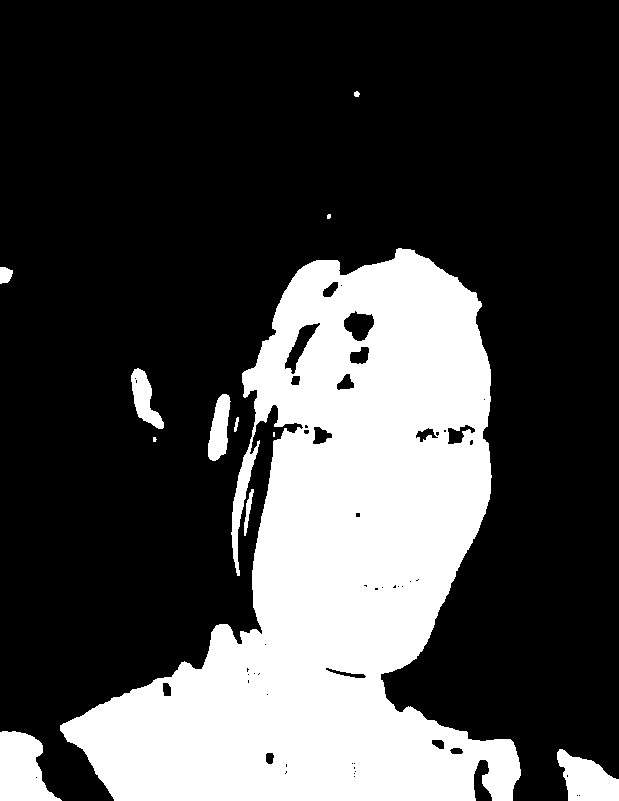
\includegraphics[width=0.2\textwidth]{Figures/chap1/EGGER_Segmentation_Nr_19.png}} \\
		\end{tabular}
	\end{center}
	\caption{It's obvious that the initial segmentation doesn't include the whole face region. Striking in this sample image are not only the eyes as mentioned before but also the shadow of the nose, which is first segmented as a background. Only after a certain number of iterations these errors are partially recognized and provided with the correct label.}
	\label{fig:iterations}
\end{figure}

\begin{figure}
	\centering
	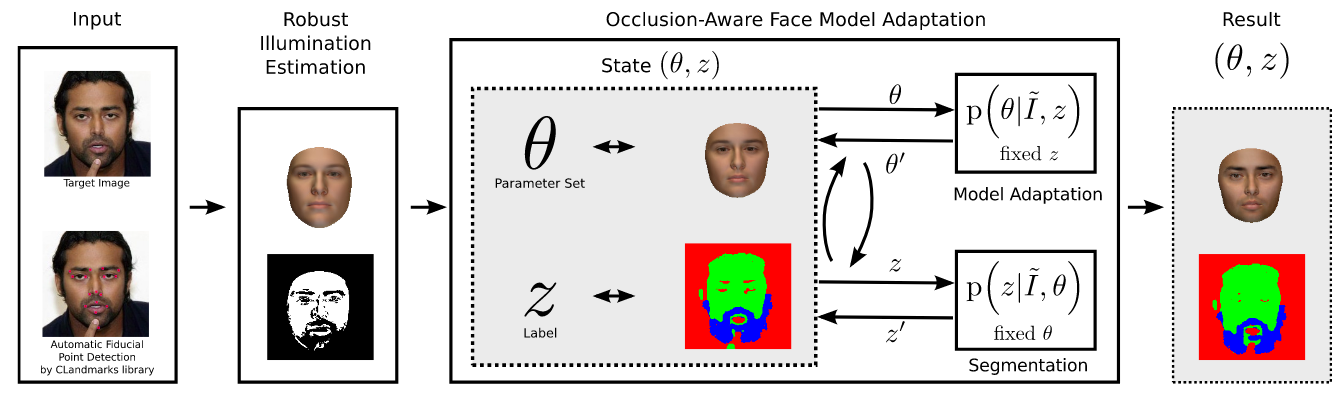
\includegraphics[width=1\linewidth]{Figures/chap1/EGGER's_method.png}
	\caption[caption without footnote, for lof]{\footnotemark Algorithm overview: As input, we need a target image and fiducial points. We use the external Clandmark Library for automated fiducial point detection from still images (U\v ri\v c\' a\v r et al (2015) \cite{Uricar}). We start with an initial face model fit of our average face with a pose estimation. Then we perform a RANSAC-like robust illumination estimation for initialization of the segmentation label z and the illumination setting (for more details see Figure 9). Then our face model and the segmentation are simultaneously adapted to the target image I. The result is a set of face model parameters $\Theta$ and a segmentation into face and non-face regions. The presented target image is from the LFW face database (Huang et al. (2007))}
	\label{fig:EGGER's_method}
\end{figure}

\footnotetext{Figure \ref{fig:EGGER's_method} and it's description are one to one coped from Fig.4 of the following paper \cite{egger_paper}}

An approach using convolutional neural networks to segment occluded faces has already been described by \cite{SaitoEtAl}. The big difference to our approach is that multiple frames are needed for the final segmentation. An other approach of \cite{MorelForster} integrate occlusion into the fitting process to model an uncertainty. They use random forests to detect facial-occlusions by hair.

\section{Expectations of the FCN}
Because \cite{nirkin2018_faceswap} trained the FCN on a very large and diverse dataset, we expect the network to perform well in the task of segmenting a face. They claim that a standart segmentation network is sufficient to segment as well as a network especially tailored for this task and outperforms state of the art methods for face segmentation. We create multiple synthetic faces and render various occlusions over them. We expect the FCN to do well on usual facial-occlusions (eg. hands, microphones) and especially on very thin occlusions, as this is a weak point of Egger's algorithm \cite{egger_paper}.\\
\\
\\
As mentionned before, the approach of Egger et al. is iterative. Due to the high resolution of the Basel Face Model and the use of a software renderer they need up to 25 minutes per image. The performance of the code was less important to them.  According to Egger et al. the runtime for the segmentation is about 2 minutes. Nirkin et al. claim that the FCN they trained surpasses previous results in both accuracy and speed. Our measurements showed an average speed of 3.2 seconds per image, including the initialisation of the FCN (on an Intel Xeon E7 v3/Xeon E5 v3/Core i7 DMI2 (rev 02)). So we expect the segmentations of the FCN to be qualitatively nearly as good as the segmentations of Egger et al. but to be much faster.